% !TEX root = main.tex
\documentclass[11pt]{article}

\newcommand{\studentname}{Your Name}
\newcommand{\studentid}{00000000}
\newcommand{\unitcode}{ENG1005}
\newcommand{\assignmenttitle}{Mathematics Assignment Template}
\newcommand{\institution}{Monash University}
\newcommand{\semester}{Semester 1, 2026}
\newcommand{\abstracttext}{%
This document is a reusable mathematics assignment template. Replace this
abstract with a short summary of the methods, results, and conclusions that
belong to the submitted work.%
}

\usepackage[a4paper,margin=1in]{geometry}
\usepackage{amsmath}
\usepackage{amssymb}
\usepackage{amsthm}
\usepackage{array}
\usepackage{booktabs}
\usepackage{caption}
\usepackage{csquotes}
\usepackage{enumitem}
\usepackage{float}
\usepackage{graphicx}
\usepackage{longtable}
\usepackage{mathtools}
\usepackage{microtype}
\usepackage{pdflscape}
\usepackage{pgfplots}
\usepackage{siunitx}
\usepackage{subcaption}
\usepackage{tabularx}
\usepackage{tikz}
\usepackage{xcolor}
\usepackage[style=apa,backend=biber]{biblatex}
\usepackage[hidelinks]{hyperref}

\addbibresource{references.bib}
\graphicspath{{figures/}}
\usetikzlibrary{arrows.meta,calc,positioning}
\pgfplotsset{compat=1.18}

\setlength{\parindent}{0pt}
\setlength{\parskip}{0.65em}
\setlist[itemize]{topsep=0.25em,itemsep=0.15em}
\setlist[enumerate]{topsep=0.25em,itemsep=0.15em}
\numberwithin{equation}{section}

\sisetup{
    detect-all,
    per-mode=symbol
}

\definecolor{monashblue}{HTML}{006DAE}
\definecolor{workinggray}{HTML}{F4F6F8}

\theoremstyle{definition}
\newtheorem{problem}{Problem}[section]
\newtheorem{definition}{Definition}[section]
\newtheorem{example}{Example}[section]

\theoremstyle{plain}
\newtheorem{theorem}{Theorem}[section]
\newtheorem{lemma}{Lemma}[section]

\theoremstyle{remark}
\newtheorem*{remark}{Remark}

\newenvironment{solution}
    {\par\noindent\textbf{Solution.}\ }
    {\hfill\(\square\)\par}

\newcommand{\todo}[1]{\textcolor{red}{\textbf{TODO:} #1}}
\newcommand{\finalanswer}[1]{\[
    \boxed{#1}
\]}

\newcommand{\R}{\mathbb{R}}
\newcommand{\N}{\mathbb{N}}
\newcommand{\Z}{\mathbb{Z}}
\newcommand{\Q}{\mathbb{Q}}
\newcommand{\C}{\mathbb{C}}

\newcommand{\vect}[1]{\mathbf{#1}}
\newcommand{\mat}[1]{\mathbf{#1}}
\newcommand{\transpose}{^{\mathsf{T}}}

\DeclarePairedDelimiter{\abs}{\lvert}{\rvert}
\DeclarePairedDelimiter{\norm}{\lVert}{\rVert}
\DeclarePairedDelimiter{\inner}{\langle}{\rangle}
\DeclarePairedDelimiter{\set}{\{}{\}}

\newcommand{\dd}{\mathop{}\!\mathrm{d}}
\newcommand{\diff}[2]{\frac{\dd #1}{\dd #2}}
\newcommand{\pdiff}[2]{\frac{\partial #1}{\partial #2}}
\newcommand{\evalat}[2]{\left.#1\right|_{#2}}



\title{\unitcode\\\assignmenttitle}
\author{\studentname\\Student ID: \studentid}
\date{\institution\\\semester}

\begin{document}

\maketitle

\begin{abstract}
\abstracttext
\end{abstract}

\tableofcontents
\newpage

% !TEX root = ../main.tex
\section{Overview}

State the assignment context, the key mathematical ideas used, and any
assumptions that affect the interpretation of later working.

\begin{definition}[Working assumption]
Record assumptions that change the domain, the units, or the validity of a
method. For example, state whether a variable is real-valued, positive, or
restricted to a measured interval.
\end{definition}

% !TEX root = ../main.tex
\section{Worked Problems}

Use this section for the main mathematical working. Keep each problem's setup,
method, calculation, and final answer close together so the reasoning is easy
to audit.

\begin{problem}[Template problem]
Let \(f(x)=x^2\). Find the derivative and evaluate it at \(x=3\).
\end{problem}

\begin{solution}
Using the power rule,
\begin{align}
    \diff{}{x} x^2 &= 2x, \\
    f'(3) &= 2(3)=6.
\end{align}

\finalanswer{f'(3)=6}
\end{solution}

\begin{problem}[Units and interpretation]
A quantity changes by \(\SI{2.5}{\metre\per\second}\) over
\(\SI{4}{\second}\). State the average rate of change.
\end{problem}

\begin{solution}
The average rate of change is
\begin{equation}
    \frac{\SI{2.5}{\metre\per\second}}{\SI{4}{\second}}
    = \SI{0.625}{\metre\per\second\squared}.
\end{equation}

\finalanswer{\SI{0.625}{\metre\per\second\squared}}
\end{solution}

% !TEX root = ../main.tex
\section{Figures and Data}

Use figures for mathematical diagrams, plots, or referenced working that is
clearer visually than in prose. Use tables for small, auditable data sets.

\begin{table}[H]
\centering
\caption{Example values for a simple quadratic}
\label{tab:example-values}
\begin{tabular}{@{}rr@{}}
\toprule
\(x\) & \(x^2\) \\
\midrule
0 & 0 \\
1 & 1 \\
2 & 4 \\
3 & 9 \\
\bottomrule
\end{tabular}
\end{table}

\begin{figure}[H]
    \centering
    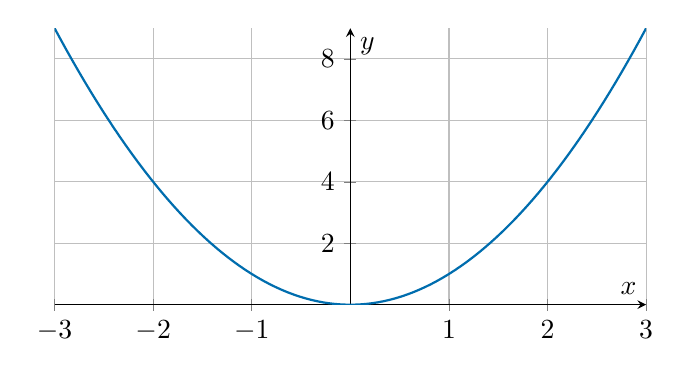
\begin{tikzpicture}
        \begin{axis}[
            width=0.75\textwidth,
            height=0.42\textwidth,
            axis lines=middle,
            xlabel=\(x\),
            ylabel=\(y\),
            grid=both,
            samples=100,
            domain=-3:3
        ]
            \addplot[monashblue, thick] {x^2};
        \end{axis}
    \end{tikzpicture}
    \caption{Example plot produced directly in LaTeX}
    \label{fig:example-plot}
\end{figure}

Refer to Table~\ref{tab:example-values} and Figure~\ref{fig:example-plot} when
discussing data or plots in the surrounding text.


% Uncomment this after adding cited sources to references.bib.
% \printbibliography

\appendix
% !TEX root = ../main.tex
\section{Supporting Material}

Use appendices for longer derivations, source data, extra plots, or other
supporting material that should not interrupt the main solution flow.


\end{document}
